\subsection{Ejercicio 3}
\graphicspath{ {img/03} }

\subsubsection{Generación clave D\&H}

Para generar la clave D\&H con CT1 primero debemos iniciar la Demostración Diffie-Hellman, en la opción Protocolos, dentro de la pestaña Procedimientos Individuales.
Esto abrirá la pantalla de la figura \ref{fig:inicioD&H}.

\begin{figure}[H]
    \centering
    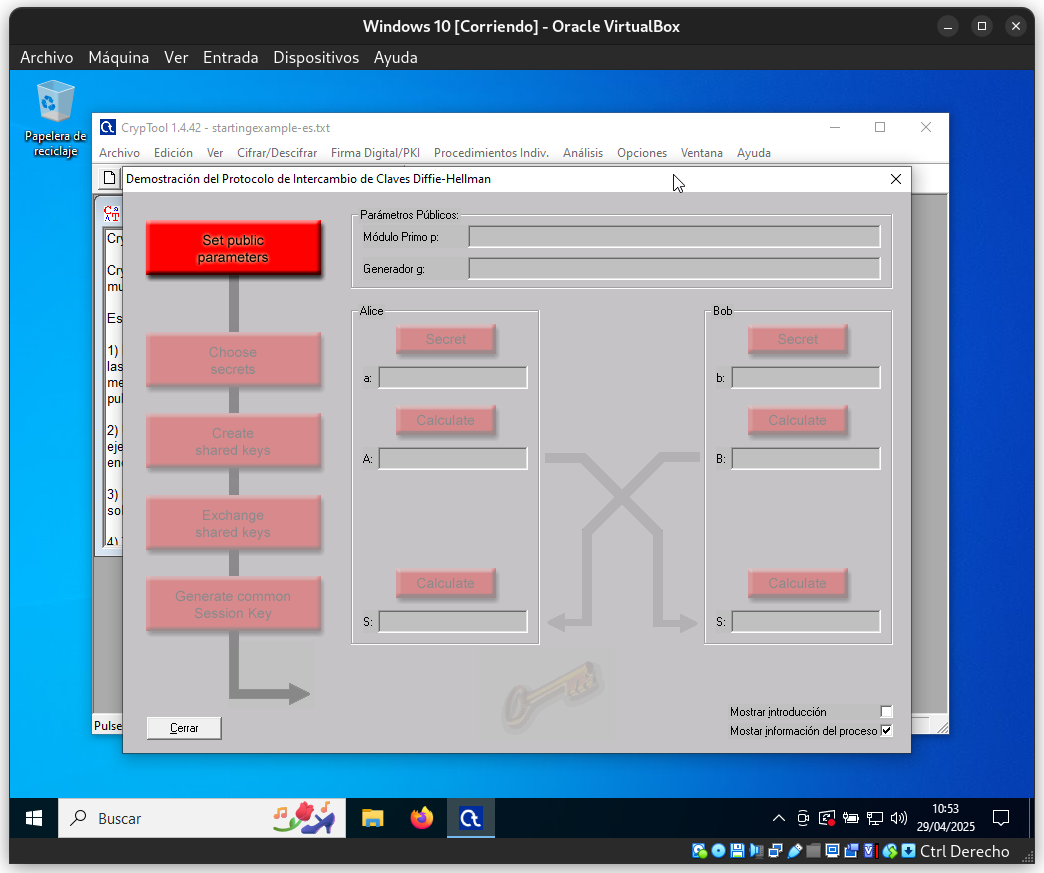
\includegraphics[width=0.8\textwidth]{D&H-1.png}
    \caption{Inicio de la simulación Diffie-Hellman}
    \label{fig:inicioD&H}
\end{figure}

Ahora, escogemos los parámetros públicos $p$, el número que hará de módulo y $g$ $(<p)$, la base del exponente (figura \ref{fig:publicparams}).

\begin{figure}[H]
    \centering
    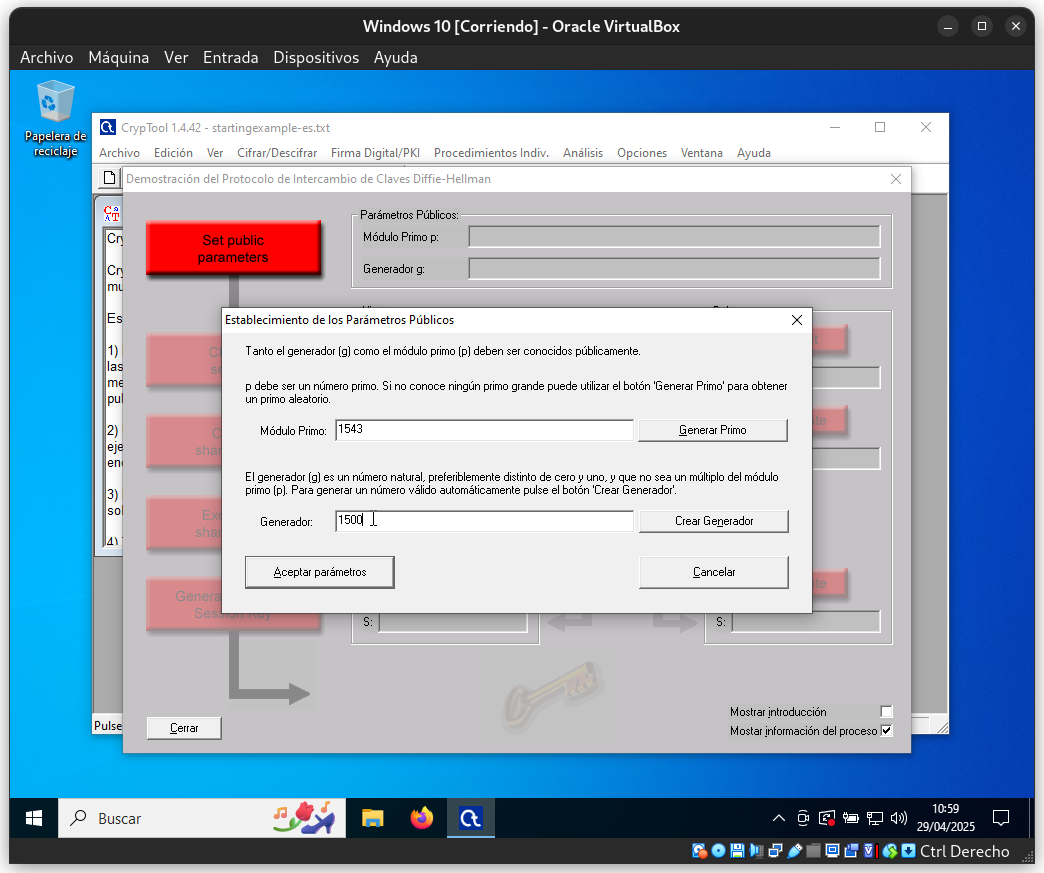
\includegraphics[width=0.8\textwidth]{D&H-2.png}
    \caption{Elección de los parámetros públicos}
    \label{fig:publicparams}
\end{figure}

El siguiente paso es que ambas partes del intercambio escojan dos números $a$ y $b$ respectivamente, como en las figuras \ref{fig:aparam} y \ref{fig:bparam}.

\begin{figure}[H]
    \centering
    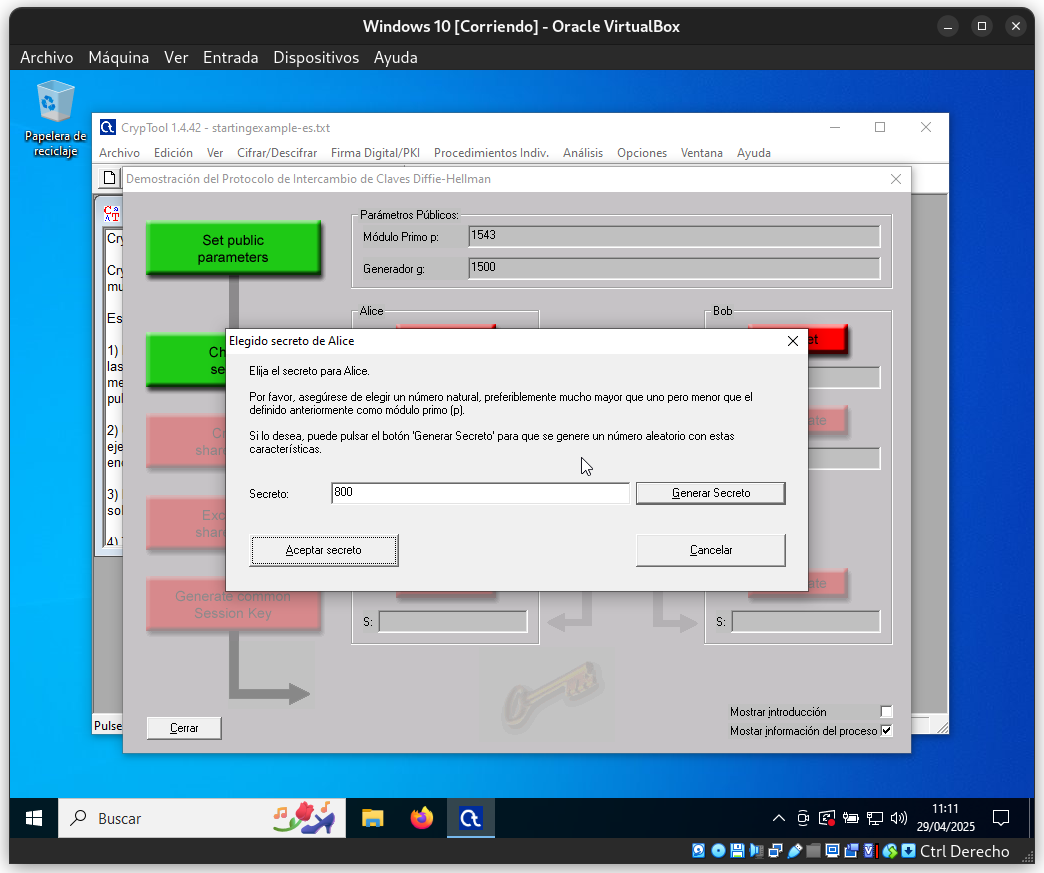
\includegraphics[width=0.8\textwidth]{D&H-3.png}
    \caption{Elección del parámetro secreto 'a'}
    \label{fig:aparam}
\end{figure}

\begin{figure}[H]
    \centering
    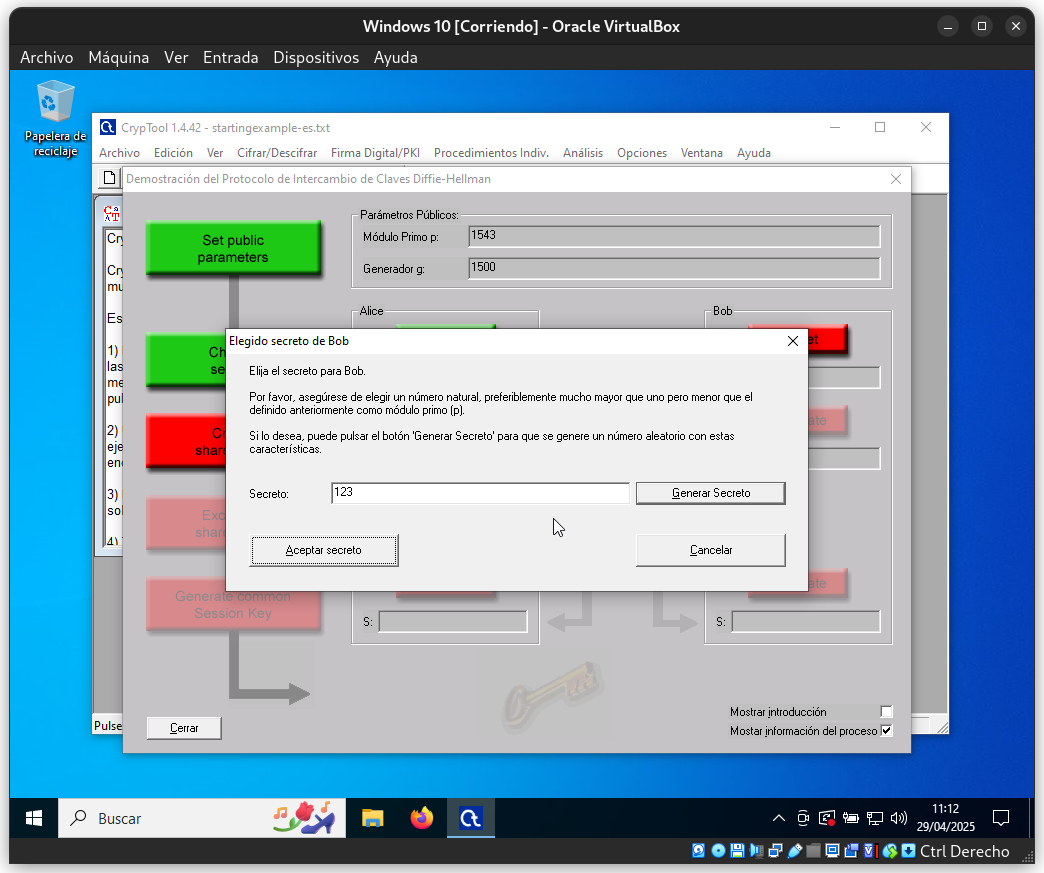
\includegraphics[width=0.8\textwidth]{D&H-4.png}
    \caption{Elección del parámetro secreto 'b'}
    \label{fig:bparam}
\end{figure}

A continuación, cada parte calcula $g^a\mod{p}$ o $g^b\mod{p}$, según tenga $a$ o $b$ y la envía a la otra parte (figura \ref{fig:modulos}).

\begin{figure}[H]
    \centering
    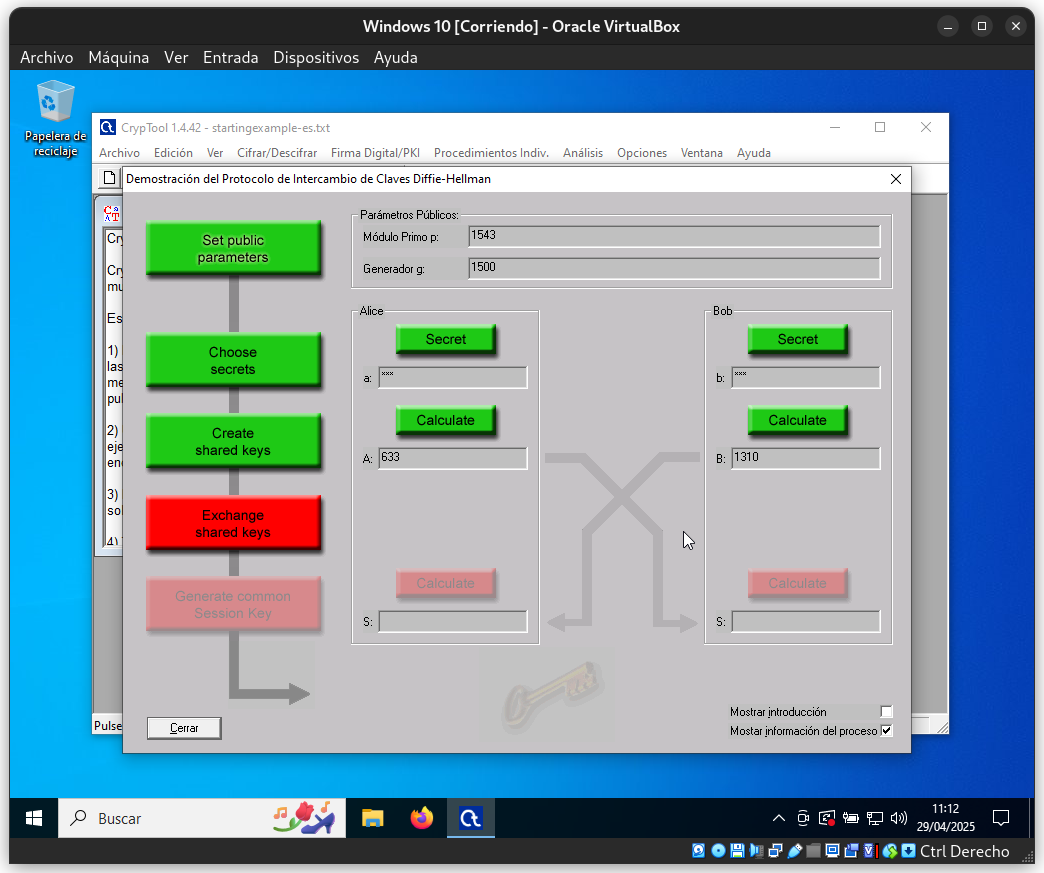
\includegraphics[width=0.8\textwidth]{D&H-5.png}
    \caption{Cálculo de $g^a\mod{p}$ y $g^b\mod{p}$}
    \label{fig:modulos}
\end{figure}

Finalmente, dados $g^a\mod{p}$ o $g^b\mod{p}$, cada parte puede calcular $g^{ab}\mod{p}$, elevando lo que recibió a su clave privada, de manera que ambos obtienen la misma clave, como se observa en la figura \ref{fig:gabmodp}.

\begin{figure}[H]
    \centering
    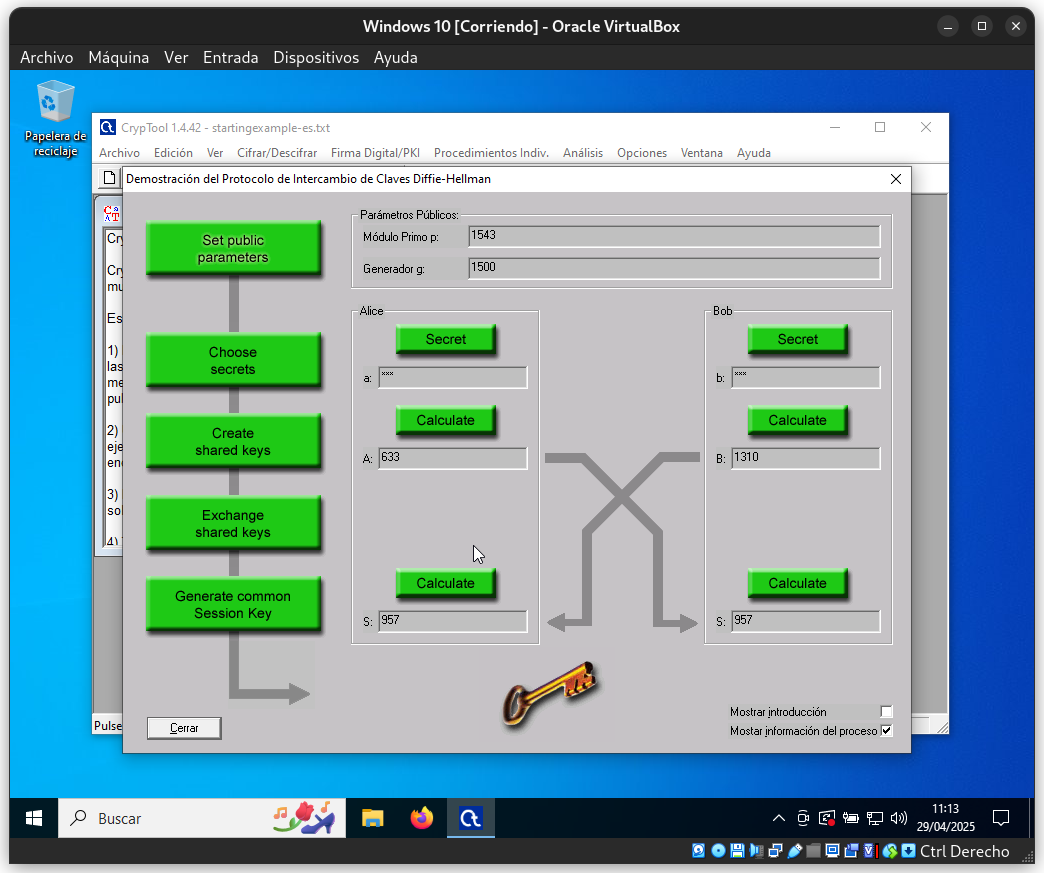
\includegraphics[width=0.8\textwidth]{D&H-6.png}
    \caption{Cálculo de $g^{ab}\mod{p}$}
    \label{fig:gabmodp}
\end{figure}


\subsubsection{Utilidad clave}

La clave generada mediante el protocolo D\&H (Diffie-Hellman) se usa para establecer un secreto compartido entre dos usuarios, incluso si se comunican a través de un canal inseguro como Internet. Este secreto compartido puede servir, por ejemplo, como clave simétrica para cifrar y descifrar mensajes. 

La funcionalidad de D\&H no es el cifrado de mensajes, sino permitir a las dos partes acordar una clave secreta. 


\subsubsection{Problemas de seguridad}

A pesar de parecer ser un método inteligente para el acuerdo de una clave secreta, si no se toman las medidas de seguridad necesarias, puede llegar a ser un método vulnerable.  

Consideramos que el principal problema con el que nos podemos encontrar es que, como D\&H no autentica las partes participantes, un atacante puede interceptar los valores públicos y establecer claves falsas con ambas partes. Así, el atacante podrá leer y modificar los mensajes sin ser detectado. 

Esto se puede solucionar utilizando distintos tipos de métodos de autenticación, como certificado digital o firma digital, para verificar las identidades participantes. 

Por otra parte, si usamos parámetros débiles como un ‘p’ muy pequeño, como es nuestro caso, se hace posible un ataque por fuerza bruta o logaritmo discreto usando computadoras modernas. 

Esto se puede evitar haciendo uso de claves suficientemente grandes, así como valores seguros de ‘p’ y de ‘g’. 
